\documentclass{article}
\begin{document}
\section{Media Transfer Protocol (MTP) firmware for APP3.x}

The external memory chip W25M02/W25N02 on APP3.x is based on NAND flash.

FAT filesystem on NAND flash memory results in a complicated solution which uses of lot of RAM. Moreover use of FAT without Flash Translation Layer (to save RAM) wears out NAND flash with frequent usage. Hence the choice of \href{https://github.com/conservify/FLogFS}{FlogFS}, a filesystem optimized for use with NAND flash.

But the use of `FlogFS`, presents a new problem 'Filesystem access from PC via USB'. Use of `FlogFS` with USB Mass Storage protocol is not possible because operating system can't recognize `FlogFS` as a valid filesystem.

Use of custom protocol to do filesystem operations would mean re-inventing the wheel and a lot of effort. User also would not have the same experience as with USB Mass Storage.

Solution was to go with the "Media Transfer Protocol" developed initially by Microsoft for Portable Devices like MP3 players. Starting from Android Kitkat (v4.4), MTP is the only way to access files on an Android device since the whole flash memory (included user storage space) uses filesystems like ext4, YAFFS, F2FS, etc.,

Files in APP3.x's NAND flash memory can be viewed using the USB MTP firmware.

Supported on Windows, Linux, macOS and Android (via USB OTG).

\begin{figure}[H]
	\begin{center}
		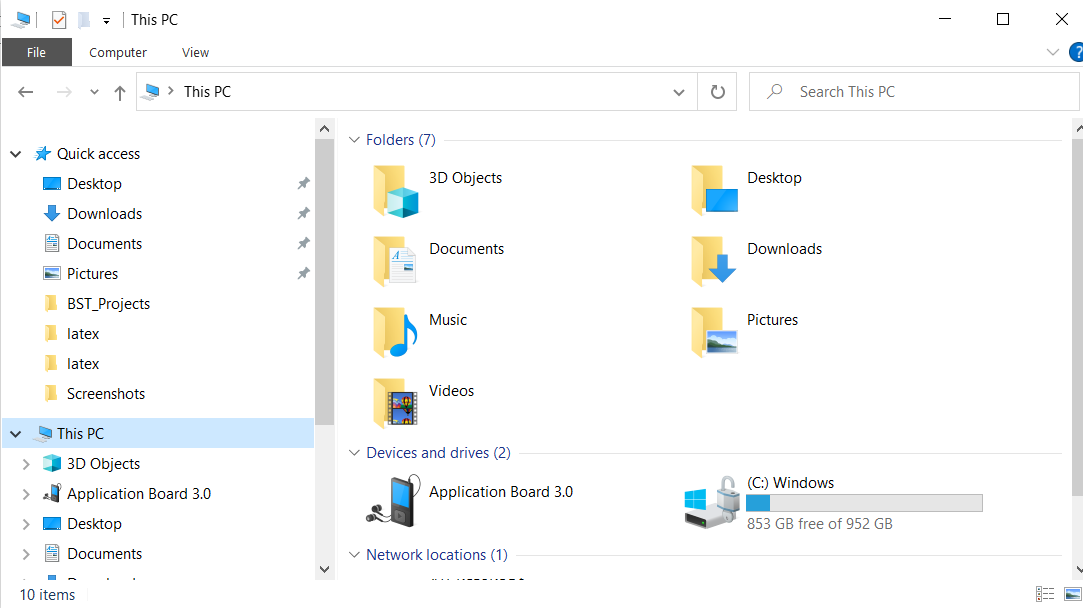
\includegraphics[width=0.7\textwidth]{coinesAPI_images/MTP_windows.png}
		\caption{APP3.x in MTP mode on Windows}
	\end{center}
\end{figure}

\begin{figure}[H]
	\begin{center}
		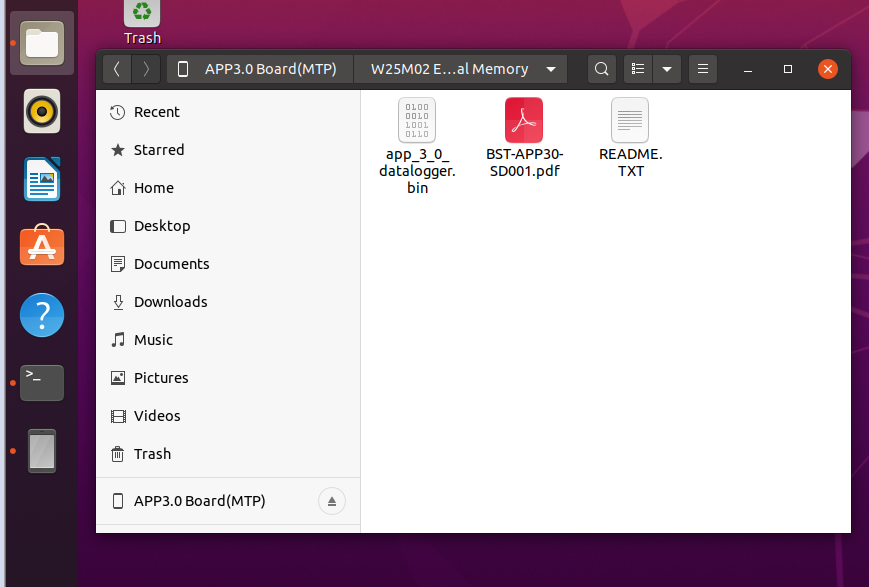
\includegraphics[width=0.7\textwidth]{coinesAPI_images/MTP_Ubuntu_Nautilus.png}
		\caption{APP3.x in MTP mode on Linux}
	\end{center}
\end{figure}

\begin{figure}[H]
	\begin{center}
		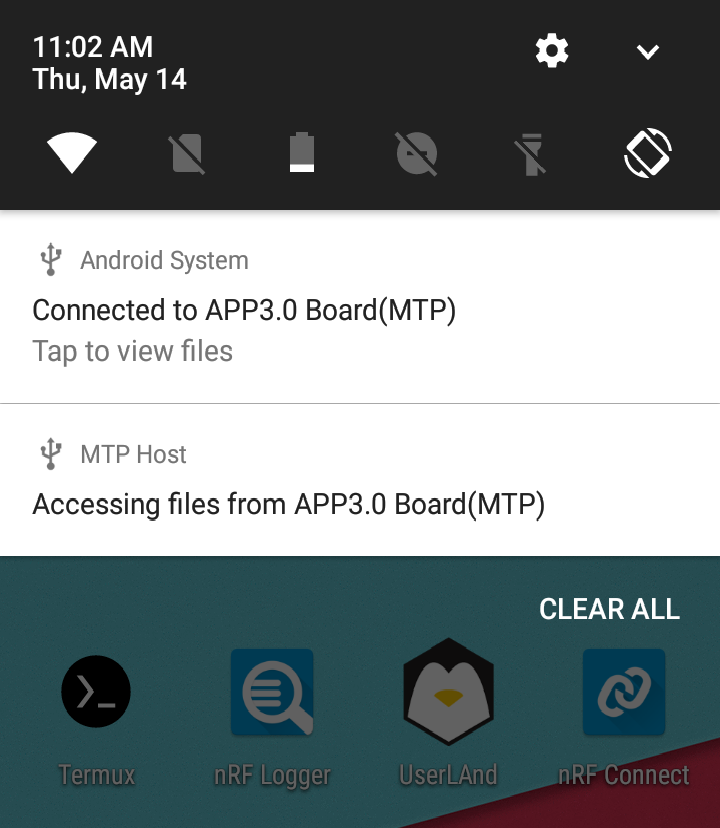
\includegraphics[width=0.5\textwidth]{coinesAPI_images/MTP_Android_2.png}
		\caption{APP3.x in MTP mode on Andriod}
	\end{center}
\end{figure}

\begin{figure}[H]
	\begin{center}
		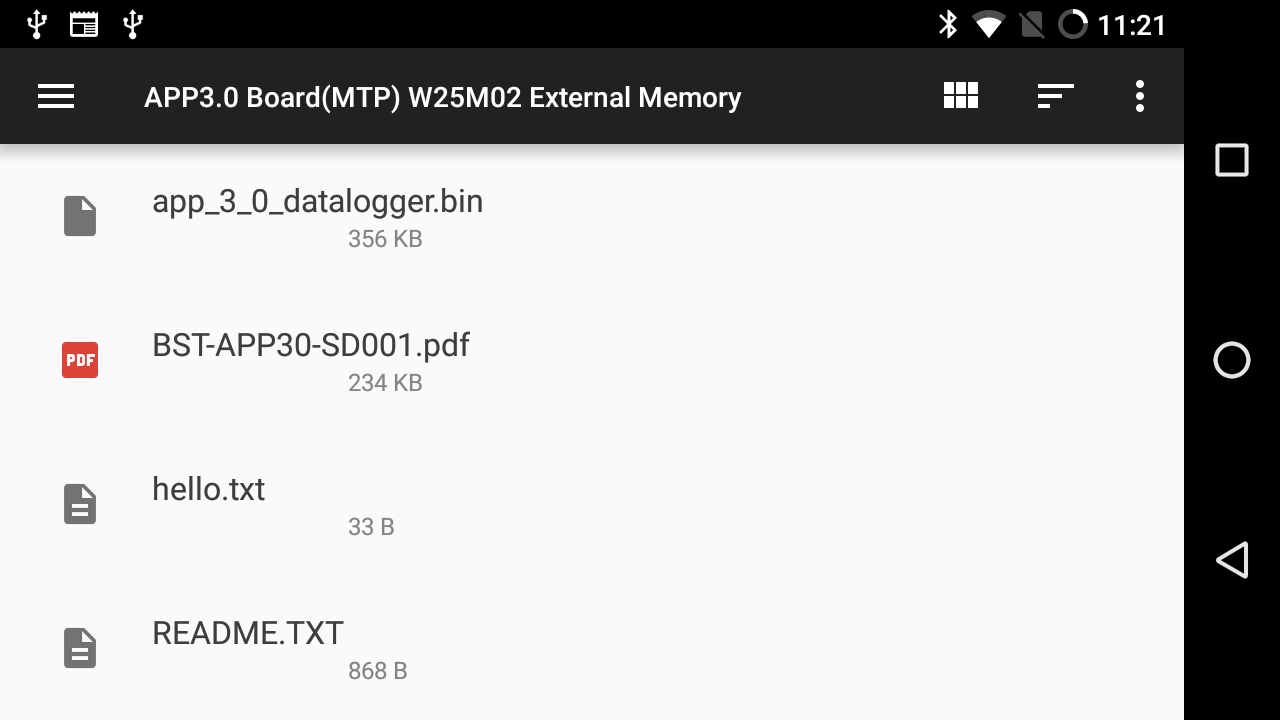
\includegraphics[width=0.7\textwidth]{coinesAPI_images/MTP_Android_3.png}
		\caption{Files in external memory listed on Andriod device}
	\end{center}
\end{figure}

\subsection{Copying the files using MTP}
The following procedure demonstrates how to copy files using MTP:
\begin{itemize}
	\item APP3.x comes with the preloaded MTP firmware update package.
	\item Refer to section \ref{SwitchModes} to switch to MTP mode
	\item The device will enumerate as an MTP device with name "Application Board 3.x". Click on it and select the "W25M02 External Memory"
	\item The device will list all the available files and all required files can be copied.
\end{itemize}

\begin{figure}[H]
	\begin{center}
		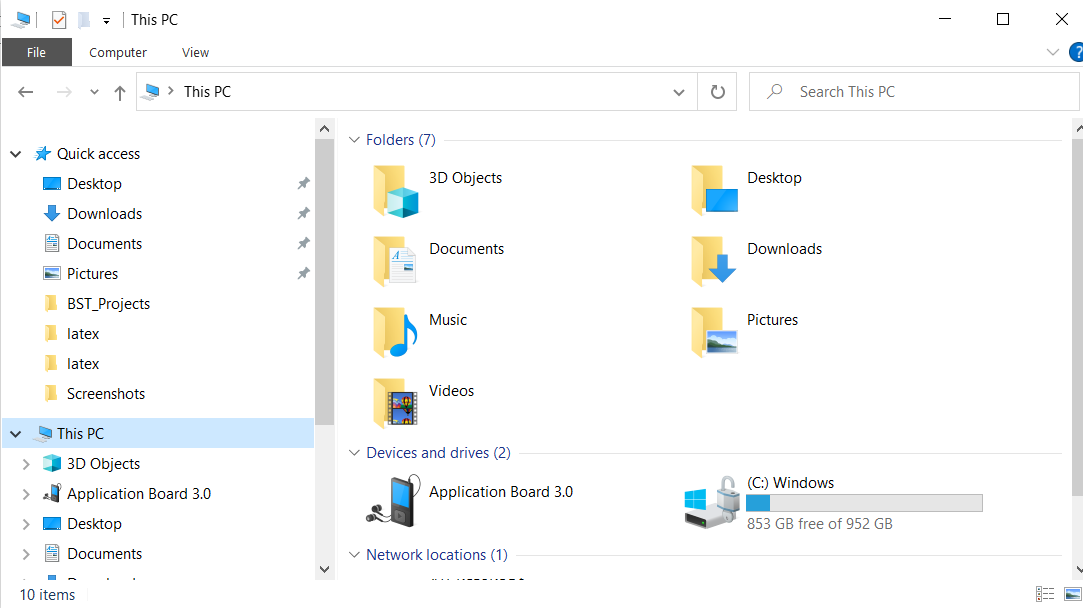
\includegraphics[width=0.7\textwidth]{coinesAPI_images/MTP_windows.png}
		\caption{Copy data log files to the PC over USB MTP}
	\end{center}
\end{figure}

\newpage

\end{document}